\documentclass[xcolor=dvipsnames]{beamer}
\usepackage{algorithm}
\usepackage{algorithmic}
\usepackage[]{natbib}
\usepackage{alltt}
\usepackage{graphicx}

% Setup appearance:

%\usetheme{Madrid}
\usetheme{Copenhagen}
\usefonttheme[onlylarge]{structurebold}
\usecolortheme[RGB={0,63,135}]{structure} 
\setbeamercolor{normal text}{fg=Black}
\setbeamerfont*{frametitle}{size=\normalsize,series=\bfseries}
%\setbeamertemplate{navigation symbols}{}

% Standard packages

\usepackage[english]{babel}
%\usepackage[latin1]{inputenc}
%\usepackage{times}
%\usepackage[T1]{fontenc}
%\usepackage{nnfootnote}
\usepackage{amsfonts}
\usepackage{amsmath}
\usepackage{xspace}

%\newcommand{\argmax}{\operatornamewithlimits{argmax}}
\def\newblock{\hskip .11em plus .33em minus .07em}
\newcommand\midtilde{{\lower.50ex\hbox{\texttt{\char`\~}}}}

% Author, Title, etc.

\title[YAPPL] 
{
  YAPPL\\
  Yet Another Probabilisitic\\ Programming Language \\
}


\author[Hu, Huggins, Hyttinen, \& McGrew]
{
  David~Hu\\
  Jonathan~Huggins\\
  Hans~Hyttinen\\
  Harley~McGrew\\
}

\institute[Columbia University]
{
  %\inst{1}%
  Columbia University
}

\date[December, 2011]
{December, 2011}

\begin{document}

%\nofootnotemark
\begin{frame}
  \titlepage
\end{frame}


\frame[t] {
\frametitle{Overview: Introduction}
Inspiration: functional,  {\bf probabilistic programming languages}
\begin{itemize}
\item {\bf Church}: PPL based on pure subset of Scheme
\item HANSEI: PPL based on Ocaml
\item OCaml: inspiration for syntax
\end{itemize}
Church and HANSEI code can be difficult to read and understand 
}


\frame[t] {
\frametitle{Overview: Probabilistic Programming}
What is probabilistic programming about?
\begin{itemize}
\item allows for the concise definition of complex statistical models
\item in particular, we are interested in defining generative {\bf Bayesian models} and conditionally sampling from them
\item to accomplish these goals, use {\bf conditional evaluation} and {\bf memoization}
\item a memoized function remembers what value it returned for previously evaluated argument values and always returns the same value in the future given those arguments 
\item memoization is useful because it lets you have "infinite" things (like lists or matrices), but only {\bf lazily generate} items from the list 
\end{itemize}
}

\frame[t] {
\frametitle{Overview: Goals}
Improving on HANSEI and Church by...
\begin{itemize}
\item implementing a functional, natively probabilistic programming language with modern, Ocaml-like syntax
\item build conditional evaluation and memoization directly into the language
\item making syntax cleaner and more readable
\end{itemize}
}

\begin{frame}[fragile]
\frametitle{Tutorial 1}
tutorials/add.ypl
\begin{alltt}
fun int:add int:a int:b = 
   a + b
in 
  {\midtilde}print_line {\midtilde}add 1 2
\end{alltt}
\end{frame}

\begin{frame}[fragile]
\frametitle{Tutorial 2}
tutorials/geom\_cond.ypl
\begin{alltt}
 {\midtilde}seed;
 fun int:geom float:q =
   fun int:geom_helper float:orig_q int:i =
     if {\midtilde}rand < orig_q then i
     else {\midtilde}geom_helper orig_q (i+1)
   in 
     {\midtilde}geom_helper q 1
 in
\end{alltt}
\end{frame}

\begin{frame}[fragile]
\frametitle{Tutorial 3}
\begin{alltt}
 fun int:try_g = {\midtilde}geom 0.1 given $ > 100 in
 {\midtilde}print_line {\midtilde}try_g;
 {\midtilde}print_line {\midtilde}try_g;
 {\midtilde}print_line {\midtilde}try_g;
 {\midtilde}print_line {\midtilde}try_g;
 {\midtilde}print_line {\midtilde}try_g;
 
 fun int:try_g2 = {\midtilde}geom 0.1 given $ > 10 in
 {\midtilde}print_line {\midtilde}try_g2;
 {\midtilde}print_line {\midtilde}try_g2;
 {\midtilde}print_line {\midtilde}try_g2;
 {\midtilde}print_line {\midtilde}try_g2;
 {\midtilde}print_line {\midtilde}try_g2
\end{alltt}
\end{frame}

\frame[t] {
\frametitle{Block Diagram}
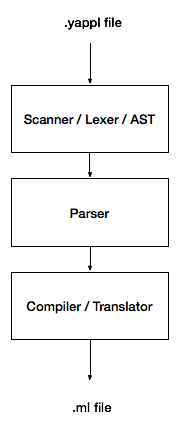
\includegraphics[scale=0.5]{block-diagram.png}
}

\begin{frame}[fragile] 
\frametitle{YAPPL code conversion to AST}
\begin{alltt} 
fun int:t1 int:a =
    a + 3
in
~print_line ~t1 2 
\end{alltt}

\end{frame}

\begin{frame}[fragile]
\frametitle{YAPPL code conversion to AST}
\begin{alltt}
FuncBindings
    FuncBind =
        FuncDecl(t1, ValType(Int), Decl(a, ValType(Int))
        Binop +
            Id a
            IntLit 3
    Eval print_line
        Eval t1
            IntLit 2
            Noexpr
        Noexpr

\end{alltt}
\end{frame}

\frame[t] {
\frametitle{Code Generation}

 {\bf Important steps}

\begin{itemize}
  \item Generate symbol table
     \begin{itemize}
        \item tracks identifiers and type
        \item can point to parent symbol table for scoping
     \end{itemize}
  \item expr\_to\_string
     \begin{itemize}
        \item main function for evaluation of ast
        \item resolves reserved identifiers before using symtable
     \end{itemize}
  \item Compile OCaml to executable
      \begin{itemize}
         \item links with builtin (includes functions like rand)
      \end{itemize}  
\end{itemize}
}

\frame[t] {
\frametitle{Summary}
\begin{itemize}
\item Yet Another Probabilisitic Programming Language, but
\begin{itemize}
\item Cleaner syntax
\item Built-in constructs: memoization, conditionals
\end{itemize}
\item \texttt{.ypl} $\rightarrow$ translation $\rightarrow$ \texttt{.ml} $\rightarrow$ execution
\begin{itemize}
\item Condensed: \texttt{./yapplc program.ypl ; ./program}
\end{itemize}
\end{itemize}
}

\frame[t] {
\frametitle{Summary}
{\bf Lessons learned}
	\begin{itemize}
	\item Start early
	\item Parallelize work structure
	\item Project scope
		\begin{itemize}
		\item Big: potential to do cool stuff
		\item Small: it will probably actually work
		\end{itemize}
	\item Unit testing 
	\item Learn debug tools
	    \begin{itemize}
	    \item OCAMLRUNPARAMS
	    \item ocamlyacc -v
	     \end{itemize}
	\end{itemize}
}

\end{document}
